%%%%%%%%%%%%%%%%%%%%%%%%%%%%%%%%%%%%%%%%%%%%%%%%%%%%%%%%%%%%%%%%%%%%%%%%%%%%%%%%%%%%%%%%%
% Section 5: Xilinx Designs
%	This section contains a description of the following:
%	- Vivado FPGA designs and netlists (with terminology)
%	- Design data structures in RapidSmith2, 
%	- Cell Libraries and how to generate new cell libraries  
%%%%%%%%%%%%%%%%%%%%%%%%%%%%%%%%%%%%%%%%%%%%%%%%%%%%%%%%%%%%%%%%%%%%%%%%%%%%%%%%%%%%%%%%%
\newpage
\section{Designs}
\graphicspath{{./techReportFigures/sec5_designs/}}

%%%%%%%%%%%%%%%%%%%%%%%%%%%%%%%%%%%%%%%%%%%%%%%%%%%
% Xilinx Netlist Structure
%%%%%%%%%%%%%%%%%%%%%%%%%%%%%%%%%%%%%%%%%%%%%%%%%%%
\subsection{Xilinx Netlist Structure} \label{sec:xilinxNetlist}
During the synthesis stage of implementation, a digital circuit expressed using
RTL (VHDL, Verilog, or SystemVerilog) is translated to a lower-level Xilinx
netlist. This netlist describes a digital circuit in terms of primitive elements
that can directly target hardware on a Xilinx FPGA. In terms of granularity, a
Xilinx netlist is more abstract than gates and transistors, but more detailed
than RTL. A list of valid primitives that can be used within a Xilinx netlist
can be found
\href{http://www.xilinx.com/support/documentation/sw_manuals/xilinx2016_2/ug953-vivado-7series-libraries.pdf}{\color{blue}{here}}
for Series7 devices and
\href{http://www.xilinx.com/support/documentation/sw_manuals/xilinx2014_1/ug974-vivado-ultrascale-libraries.pdf}{\color{blue}{here}}
for Ultrascale devices. The primitives of a Xilinx netlist are wired together to
create a digital circuit capable of being implemented on a FPGA.
\autoref{fig:schematic} shows an example netlist for a 3-bit counter created in Vivado.

\begin{figure}[h!]
 \centering
 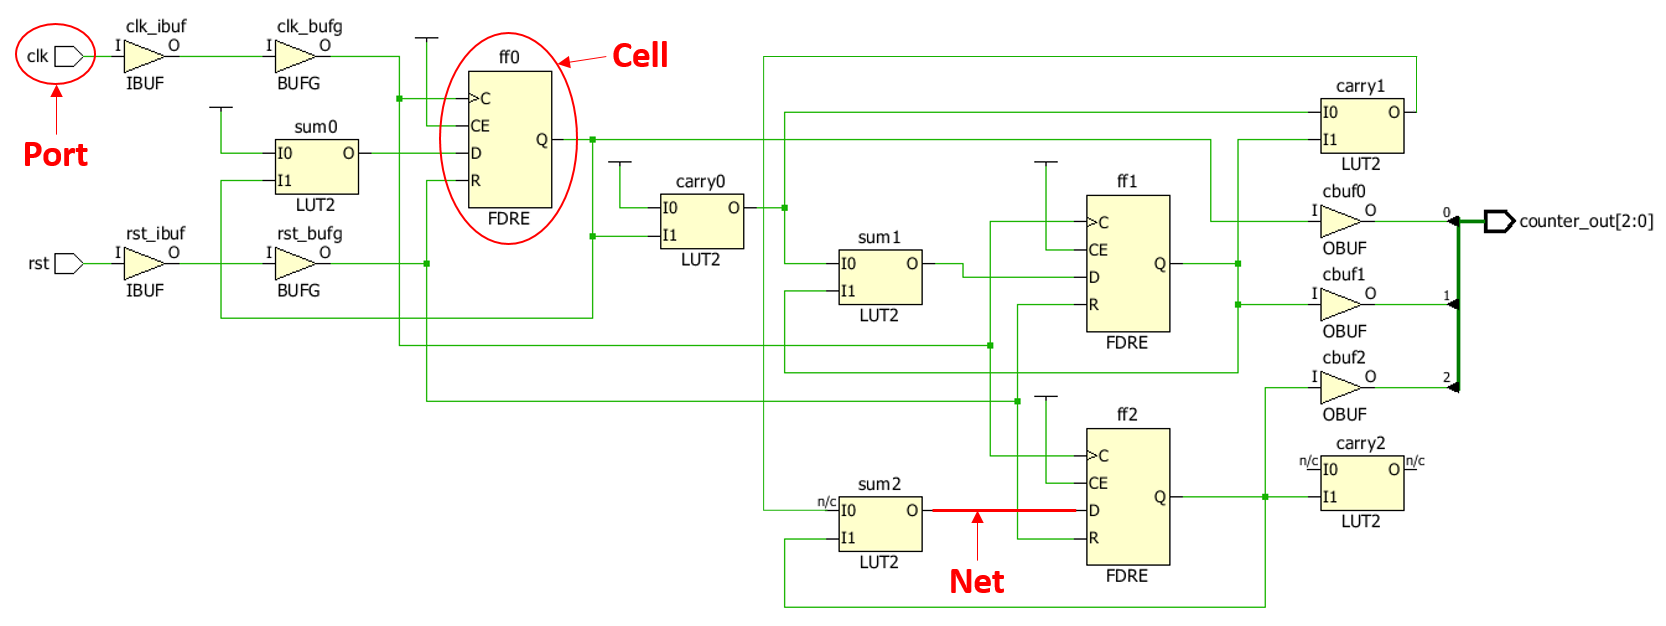
\includegraphics[width=1\columnwidth]{schematic.png}
 \caption{Schematic of a 3-bit counter in Vivado using LUT and FDRE cells.
 The yellow boxes are cells, the green lines are nets, and and the
 white figures on the edge of the diagram are ports.}
 \label{fig:schematic}
\end{figure}

As the figure shows, Vivado netlists are composed of three primary components:
\texttt{Cell}s, \texttt{Net}s, and \texttt{Port}s. Cells are \textbf{instances} of
Xilinx primitives. They are the basic building blocks of a Xilinx netlist and
implement the actual logic of a digital design. The most commonly used
cells include:

\begin{itemize}
  \item \textbf{Look Up Tables} (LUTs): Implement logic equations such as
  $O6 = (A1 + A2) \oplus A3$.
  \item \textbf{Flip-Flops} (FDxx): Single-bit storage elements.
  \autoref{fig:schematic} uses a FDRE cell which specifies a rising-edge
  flip-flop with a reset port, but ties the clock enable port high. Other
  types of FDxx cells can be used to include a clock enable port.
  \item \textbf{Block Ram} (BRAMs): On-chip FPGA memory.
  \item \textbf{Digital Signal Processing Units} (DSPs): Perform complex arithmetic
  functions efficiently.
  \item \textbf{Buffers} (BUF): IO, clock, and other types of signal buffers. 
\end{itemize}

\noindent
Several other types of cells can be used, but the ones in the list above
are the most common. Nets connect cells together. In
other words, the output of one cell is wired to the input of another
cell using a net. Ports are simply design input/output (IO). In terms of an FPGA
design, ports are mapped to specific peripheral pins of the FPGA
for chip IO. It is important to note that a Xilinx netlist is purely logical.
There is no physical information within the netlist (i.e. there is no information about
where the cells have been placed, or how the nets have been routed). When
exporting a design from Vivado, the Xilinx netlist representation is converted
to an electronic design interchange format (EDIF) file.

%%%%%%%%%%%%%%%%%%%%%%%%%%%%%%%%%%%%%%%%%%%%%%%%%%%
% RapidSmith2 Netlist Data Structures
%%%%%%%%%%%%%%%%%%%%%%%%%%%%%%%%%%%%%%%%%%%%%%%%%%%
\subsection {RapidSmith2 Netlist Data Structures} \label{sec:designDS}
RapidSmith2 netlists are modeled closely after Xilinx netlists. In fact,
much of the terminology between the two are identical or very similar. For those
that are familiar with Vivado designs, this should make the transition to
RapidSmith2 straightforward. The data structures that constitute a RapidSmith2
netlist can be found in the package
\textit{byu.edu.ece.rapidSmith.design.subsite}.
The package hierarchy is shown in \autoref{fig:designDS}.

\begin{figure}[H]
 \centering
 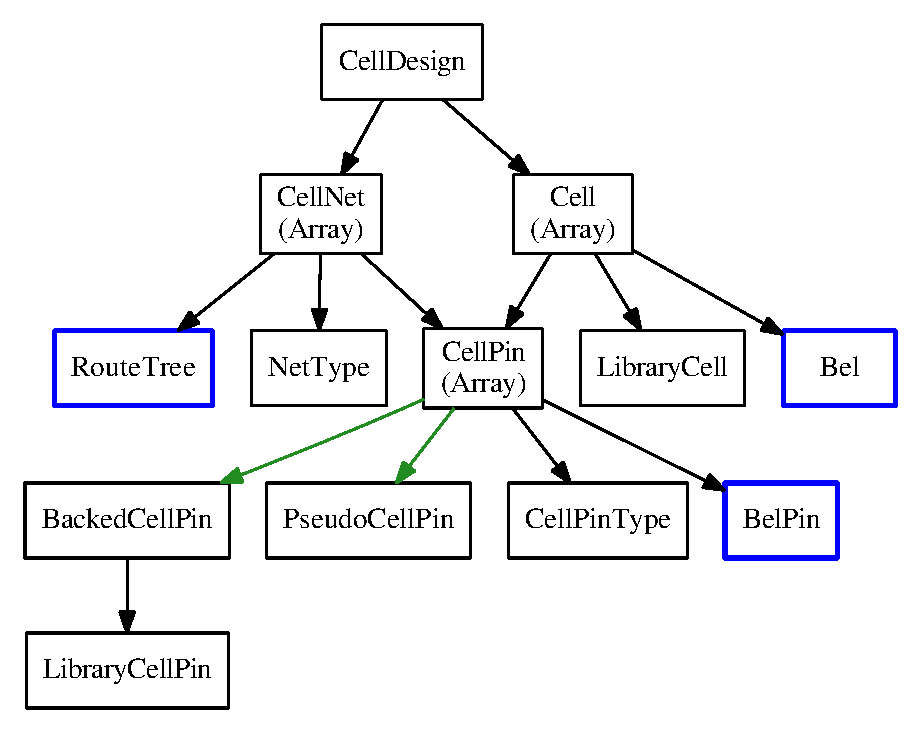
\includegraphics[width=.6\columnwidth]{designDS.eps}
 \caption{RapidSmith2 design data structure tree. Black arrows represent
 composition, green arrows represent inheritance, and blue boxes are physical
 implementation components of the netlist.}
 \label{fig:designDS}
\end{figure}

As can be seen, a \texttt{CellDesign} is the top-level design object in
RapidSmith2. It consists of a collection of \texttt{Cell} objects,
interconnected by \texttt{CellNet}s. RapidSmith2 \texttt{Cell}s are equivalent
to Xilinx cells and RapidSmith2 \texttt{CellNet}s are equivalent to Xilinx nets.
Each \texttt{Cell} has a template \texttt{LibraryCell}, which represents
a Xilinx library primitive (i.e. a LUT). They also have a collection of
connected \texttt{CellPin} objects. Placing and routing these logical design
elements is described in Section~\ref{sec:placement} and \ref{sec:routing}
respectively. The best way to learn how to utilize the classes shown in
\autoref{fig:designDS} is to generate and read through the
JavaDocs, but important aspects of each class is included in the
following subsections.


\subsubsection{CellDesign} \label{sec:cellDesignDS}
As previously mentioned, the \texttt{CellDesign} class is the top-level netlist
object in RapidSmith2. An instance of a \texttt{CellDesign} contains the
following:

\begin{itemize}
  \item A list of cells
  \item A list of nets 
  \item Global GND and VCC nets
  \item Cell placement information (i.e. where each cell is placed)
  \item The used site PIPs of each site
  \item A list of XDC constraints imported from Vivado. See Section~\ref{sec:import}
  for more information about XDC constraints and how they are represented in
  RapidSmith2.
  \item The design mode. Possible options include OUT\_OF\_CONTEXT and REGULAR.
  OUT\_OF\_CONTEXT designs are those that have been implemented in Vivado
  ``out-of-context'', meaning that the top-level ports are not placed or routed.
  Most designs are implemented in REGULAR mode.
\end{itemize}

\noindent
The \texttt{CellDesign} class has a variety of methods to retrieve and manipulate
the cells and nets of a design, place cells onto physical BELs, configure
sub-site routing, and perform several other tasks.
 
\subsubsection{Cell}
\texttt{Cell} objects are the building blocks of RapidSmith2 netlists. This
section details some important aspects of \texttt{Cell}s.

\begin {itemize}
  \item A \texttt{Cell} always contains a reference to a backing
  \texttt{LibraryCell} object. A \texttt{LibraryCell} is equivalent to a Xilinx
  primitive cell (described in Section~\ref{sec:xilinxNetlist}), and serves as a
  template for instantiated \texttt{Cell} objects. The template is used to save
  memory when creating several \texttt{Cell}s of the same type. Whenever a new
  \texttt{Cell} object is created, a corresponding \texttt{LibraryCell} must be
  specified in the constructor. \autoref{code:cells} demonstrates how to create
  new cells in RapidSmith2 and filter cells based on their type.
\end {itemize}  

\begin{lstlisting}[xleftmargin=1.5em, framexleftmargin=1.5em, caption=How to
create new cells in RapidSmith2, label=code:cells] 
// You need to have a cell library to create a cell
CellLibrary libCells = new CellLibrary(RSEnvironment.defaultEnv()
				.getPartFolderPath("xc7a100t-csg324")
				.resolve("cell_library.xml"));

// How to create a new cell. The first argument is the name of the cell, the
// second argument is the library cell
Cell cell = new Cell("myCell", libCells.get("LUT6"));

// Get all cells in a design of a certain type
CellDesign design = getCellDesign();
Stream<Cell> cells = design.getCellsOfType(libCells.get("FDRE"));
\end{lstlisting}

\begin {itemize}
  \item The method call \texttt{CellDesign::getCellsOfType(String,CellLibrary)}
  can be used to get all cells in the current design with a specific type.
  
  \item The methods \texttt{Cell::getPins()},
  \texttt{Cell::getInputPins()}, and \texttt{Cell::getOutputPins()} can be used
  to get a handle to the pins of a \texttt{Cell}. In certain special cases, more
  pins must be added to a \texttt{Cell} object.  In these cases,
  \texttt{PseudoCellPin} objects can be attached (see
  Section~\ref{sec:pseudoCellPin} for details).
  
  \item \texttt{Cell}s can be placed onto \texttt{Bel} objects of the
  current \texttt{Device}. See Section~\ref{sec:placement} for more information about
  cell placement.
  
  \item Top-level \texttt{Port}s in Vivado (design input/output) are represented as
  Port \texttt{Cell}s in RapidSmith2. Specifically, there are three types of
  port cells: IPORT, OPORT, and IOPORT. The method \texttt{CellDesign::getPorts()} can
  be used to iterate through the ports in a design, and 
  \texttt{Cell::isPort()} can be used to determine if a given \texttt{Cell} is
  actually a port.
  
  \item RapidSmith2 supports both Xilinx macro and leaf cells. More information
  about these is given in Section~\ref{sec:xilinxNetlist}.
\end{itemize}

\subsubsection{CellPin} \label{sec:cellPin}

\texttt{CellPin}s in RapidSmith2 are attached to \texttt{Cell} objects
and are equivalent to the cell pins found in Vivado. Each \texttt{CellPin}
has an associated \texttt{CellPinType} and \texttt{PinDirection}.
\autoref{tab:pinEnums} displays the possible values for both of these
properties. The \texttt{CellPinType} can be used to find all \texttt{RESET}
pins in a design, determine if a net is a clock net (it connects to pins of type
\texttt{CLOCK}), and help with other useful functions. Cell pins of type
\texttt{PSEUDO} are a special case, and described in Section~\ref{sec:pseudoCellPin}.
The \texttt{PinDirection} field is typically used to filter a list of
pins on a cell by their direction. It is especially useful for finding INOUT
pins.

\begin{table} [t!]
\caption{Cell Pin Types and Directions}
\begin{center}
\begin{tabu}{ |c|l| }
\hline
\textbf{Property} & \multicolumn{1}{|c|}{\textbf{Values}}\\
\hline
\hline
 & CLEAR \\ 
 & CLOCK  \\
 & ENABLE \\      
 & PRESET \\ 
 & RESET \\
\texttt{CellPinType} & REUSED \\
 & SET \\
 & SETRESET \\
 & WRITE\_ENABLE \\
 & DATA \\
 & PSEUDO \\
\hline
 & IN \\
\texttt{PinDirection} & OUT \\ 
 & INOUT\\ 
\hline
\end{tabu}
\label{tab:pinEnums}
\end{center}
\end{table}

\subsubsection{CellNet}
\texttt{CellNet}s are used to wire components of a logical netlist
together. Specifically, a \texttt{CellNet} connects an output \texttt{CellPin}
to several input \texttt{CellPin}s with the purpose of transferring a signal
from one \texttt{Cell} to another. \autoref{lst:cellNet} shows the basic usage
of \texttt{CellNet} objects in RapidSmith2, and the remainder of this section
details other important aspects about \texttt{CellNet}s.

\begin{lstlisting}[xleftmargin=1.5em, framexleftmargin=1.5em, caption=Basic
CellNet functions, label=lst:cellNet] 
  // get a handle to a design
  CellDesign design = getCellDesign();
	
  // creating a new net
  CellNet net = new CellNet("myNet", NetType.Wire);
  design.addNet(net); 
	
  Cell cell1 = design.getCell("cell1");
  Cell cell2 = design.getCell"cell2");
	
  // connecting nets to cell pins
  net.connectToPin(cell1.getSourcePin());
  net.connectToPin(cell2.getpin("a"));
\end{lstlisting}

  \begin{figure}[h]
   \centering
   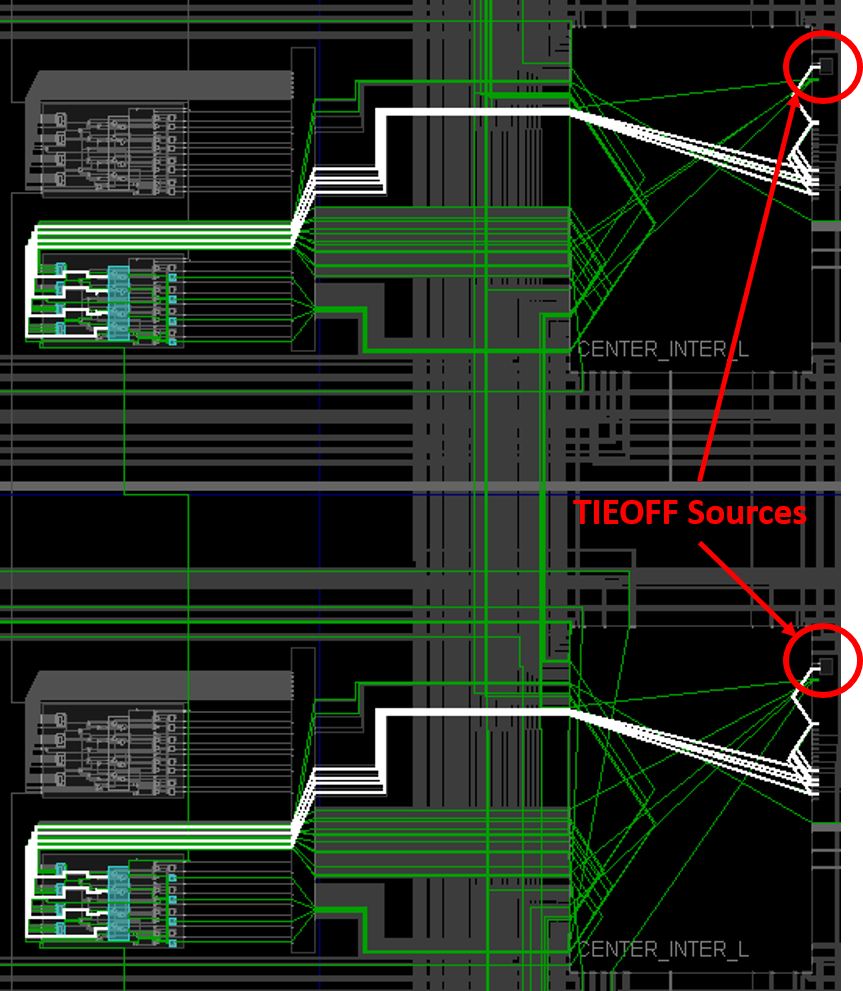
\includegraphics[width=.49\columnwidth]{staticNetSources.png}
   \caption{Example of a Vivado net with multiple sources. The highlighted
   wires in white are all part of the same net.}
   \label{fig:staticNetSources}
  \end{figure}
  
\begin{itemize}
  \item \texttt{CellNet}s are routed using \texttt{RouteTree} data structures.
  RapidSmith2 routing is described in more detail in Section~\ref{sec:routing}.
  
  \item All \texttt{CellNet}s have a \texttt{NetType} enumeration. Possible values for
  \texttt{NetType} include VCC, GND, and WIRE. VCC is reserved for power nets, GND
  is reserved for ground nets, and WIRE represents all other nets in the design.
  
  \item The suggested approach to working with static nets in RapidSmith2 is to
  have only one VCC and GND net in a \texttt{CellDesign}. In general, this
  representation is much easier to work with and the special nets
  can be obtained with the functions \texttt{CellDesign::getVccNet()}
  and \texttt{CellDesign::getGndNet()}. When a design is imported from Vivado
  through a RSCP, all VCC and GND nets are collapsed automatically. Having
  multiple VCC and GND nets, however, is still supported if desired.
  
  \item Most nets have a single driver, but some can be sourced in multiple
  locations. \autoref{fig:staticNetSources} shows an example for a GND
  net. RapidSmith2 handles this oddity by allowing \texttt{CellNet}s to have
  more than one \texttt{RouteTree} object associated with it. In the case of
  \autoref{fig:staticNetSources} the net would have two \texttt{RouteTree}s,
  one for each source TIEOFF.
  
  \item \autoref{fig:iobNet} shows a bidirectional net in Vivado. As can be
  seen, the highlighted net can be driven by both the OBUF output, and from an
  external source via the PAD BEL. RapidSmith2 supports bidirectional nets, 
  and a list of possible drivers can be obtained with the function call
  \texttt{CellNet::getAllSources()}.
  
  \begin{figure}[H]
   \centering
   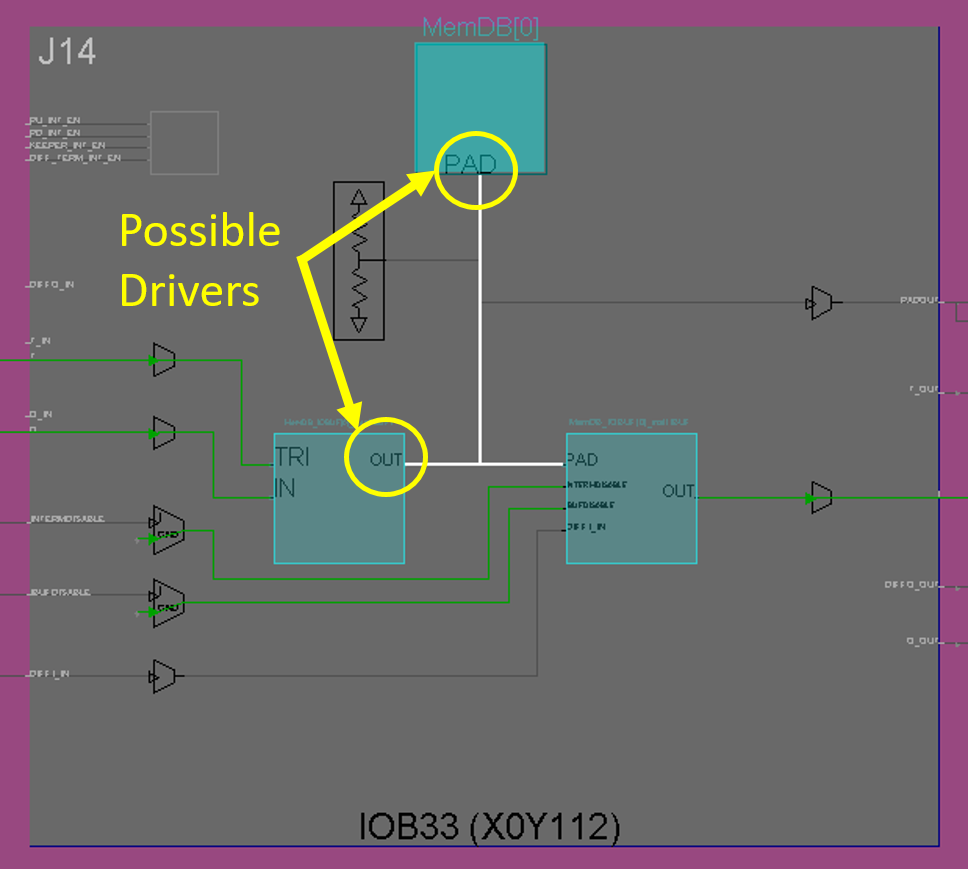
\includegraphics[width=.4\columnwidth]{iobNet.png}
   \caption{Bidirectional Net}
   \label{fig:iobNet}
  \end{figure}

 \begin{figure}[t!]
   \centering
   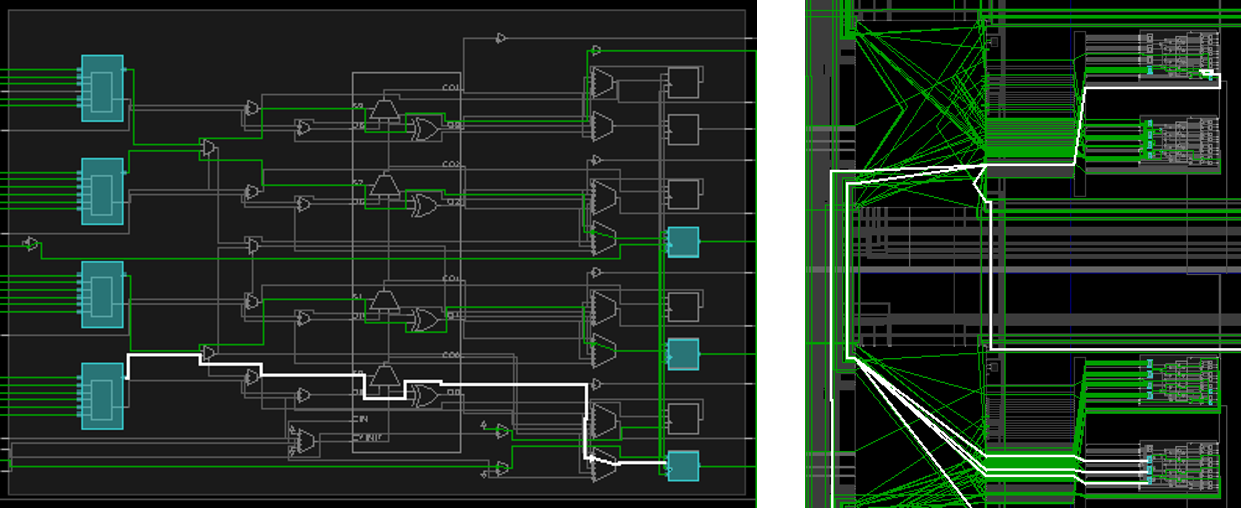
\includegraphics[width=.9\columnwidth]{interVsIntra.png}
   \caption{Example INTRASITE Net (left) and INTERSITE Net (right)}
   \label{fig:interVsIntra}
  \end{figure}
  
  \item After a design has been placed, \texttt{CellNet}s fall into one of two
  categories: \textbf{intrasite} vs. \textbf{intersite}.
  \autoref{fig:interVsIntra} shows an example of both types of nets. As can be
  seen, intrasite nets do not cross site boundaries while intersite nets stretch
  across multiple sites. To determine if a \texttt{CellNet} is an intrasite
  net, the method \texttt{CellNet::isIntrasite()} can be used. 
 
\end{itemize}

\subsubsection{Macro Cells} \label{sec:macros}

Most cells in RapidSmith2 or Vivado designs are leaf cells (LUTs, Flip Flops,
etc.), but Xilinx also supports \textbf{macro} primitives. A macro is a
hierarchical cell that groups one or more leaf cells together to perform a
specific function. An example macro is shown in \autoref{fig:macroCell} for an
IOBUF cell. An IOBUF macro cell contains two \textbf{internal} cells: one of
type OBUFT and the other of type IBUF. It also contains one internal net that
connects the two internal cells together. External cell pins of the macro
connect to one or more internal cell pins.

\begin{figure}[H]
  \centering
  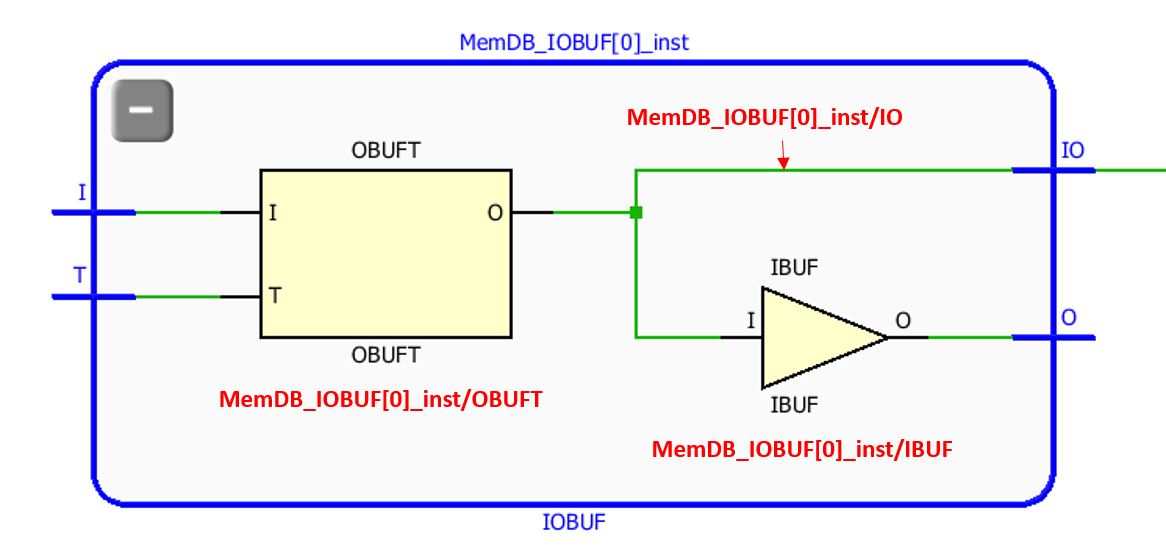
\includegraphics[width=.7\columnwidth]{macroCell.png}
  \caption{Vivado Macro Cell}
  \label{fig:macroCell}
\end{figure}

RapidSmith2 now supports importing macro cells from Vivado and adding them to a
\texttt{CellDesign}. \autoref{code:macros} gives a brief introduction to using
macros in RapidSmith2.

\begin{lstlisting}[xleftmargin=1.5em, framexleftmargin=1.5em, caption=How to use
macros in RapidSmith, label=code:macros] 
// Get a handle to a design and cell library
CellDesign design = getCellDesign();
CellLibrary libCells = getCellLibrary();

// Create a new macro cell and add it to a design
Cell macro = new Cell("myMacro", libCells.get("IOBUF"));
design.addCell(macro);

// Connect the macro cell to a net 
CellPin pin = macro.getPin("IO");
design.getNet("TmpNet").connectToPin(pin);

// Iterate through a list of all cells (macro and leaf cells) of a design
for (Cell cell : design.getCells) {
	if ( cell.isMacro() ) {
		List<Cell> internalCells = cell.getInternalCells();
		List<CellNet> internalNets = cell.getInternalNets();
		List<CellPin> externalPins = cell.getPins();
		// do something with the macro info
	}
	else {
		// do something with a regular leaf cell 
	}
}

\end{lstlisting}

\noindent
As the code example above shows, macro cells are generally used
exactly like regular leaf cells. However, there are a few distinctions
between macro cells and leaf cells.

\begin{itemize}
  \item When a macro cell is added to a design, all internal
  cells and nets are automatically added to the design as well. Users do
  not have to worry about adding these themselves. Similarly, when a macro cell
  is removed from a design, the internal cells and nets are also removed.
  
  \item When a macro cell pin is connected to a \texttt{CellNet}, RapidSmith2
  automatically connects the net to the corresponding internal pins. When a
  macro cell pin is disconnected from a \texttt{CellNet}, the internal cell pins are
  disconnected. Nets in RapidSmith2 only connect to leaf cell pins (i.e. it is
  essentially a flattened netlist with macros cell ``wrappers'').
  
  \item Internal cells and nets within a macro cannot be individually added or
  removed from a design. If this is attempted, an exception will be
  thrown. Instead, the entire macro cell must be added or removed.
  
  \item Macros cannot be placed. Rather, the internal cells of a macro should be
  placed instead.
  
  \item When a \texttt{CellDesign} is exported from RapidSmith, macro cells are not
  exported. The design is first flattened, and only the internal cells and nets
  are exported. This means the macro will not be rebuilt in Vivado, but the
  design will still be functionally equivalent.
\end{itemize}

\subsubsection {PropertyList}

\begin{figure}[t]
 \centering
 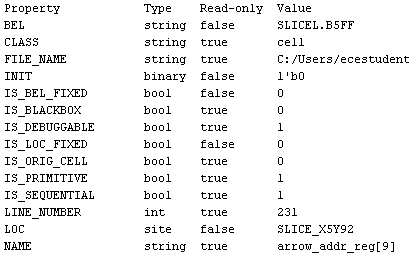
\includegraphics[width=.5\columnwidth]{vivadoProperties.png}
 \caption{Properties of a Vivado FDCE Cell}
 \label{fig:properties}
\end{figure}


Most objects in Vivado's Tcl interface have attached properties. These
properties can be used to describe attributes of the object (such as name,
type, etc.), but they can also be used for configuring the object.
\autoref{fig:properties} shows a list of properties for a FDCE flip flop
cell in Vivado. The Tcl command \texttt{[report\_property \$object]} can be used to
list all properties for a given Vivado object (cell, BEL, etc.). Cells
are the most interesting objects in terms of properties because the function
of a \texttt{Cell} is determined by how it is configured. For example, the
memory width of a BRAM cell in Vivado is configured by setting the
\texttt{READ\_WIDTH} and \texttt{WRITE\_WIDTH} properties of the cell. Possible
values include 1, 2, 4, 9, 18, 36 and 72. The operation of the BRAM is different
depending on how this property is set. Another example is a D flip flop cell
(FDRE) and its \texttt{IS\_C\_INVERTED} property. This property indicates if
the flip flop will be rising-edge or falling-edge triggered. The properties of
cells, nets, and the top-level design are included in the output EDIF netlist
of a RSCP for non-default values only.

When RapidSmith2 parses the EDIF file of a RSCP, the properties
within are stored in a data structure called a \texttt{PropertyList}. Each
\texttt{CellDesign}, \texttt{Cell}, and \texttt{CellNet} in RapidSmith has an
associated \texttt{PropertyList} object. The \texttt{PropertyList} for each
cell in the design also has a list of default configuration properties.
Configuration properties for cells are always included in the
\texttt{PropertyList} even if they are not explicitly set by the user because
the functionality of the cell is dependent on how it is configured.
\autoref{code:properties} shows some basic property usage.

\begin{lstlisting}[xleftmargin=1.5em, framexleftmargin=1.5em, caption=Using
PropertyLists in RapidSmith, label=code:properties] 
// Create a new FF cell with default properties
CellLibrary libCells = getCellLibrary();
LibraryCell libCell = libCells.get("FDRE");
Cell cell = new Cell("myCell", libCell);

// Get a handle to the cells properties
PropertyList properties = cell.getProperties();

// Print the configurable properties of the cell 
for(String propName : libCell.getConfigurableProperties()) {
	Property prop = properties.get(propName);
	System.out.println(propName + ":");
	System.out.println("\tDefault -> " + prop.getStringValue());
	System.out.println("\tPossible -> " + libCell.getPossibleValues(propName)); 
}

// Iterating over a PropertyList
for (Property prop : properties) {
	System.out.println(prop.getKey() " -> " + prop.getStringValue());
}

// Change the FF to be falling edge triggered...this will override the default
property properties.update("IS_C_INVERTED", PropertyType.EDIF, "1'b1");


\end{lstlisting}

\noindent Some additional notes about properties are given below. 

\begin{itemize}
  \item In Vivado, the configurable properties on a cell can be determined by
  using the Tcl command \texttt{[report\_prope\-rty [get\_lib\_cells \$cell]]}.
  All properties that start with ``CONFIG'' are configurable properties that
  can be modified.
  
  \item Because EDIF properties only support String, Integer, and Boolean types,
  any properties imported from the EDIF file will be one of these types.
  It seems, however, that Vivado always exports its properties as strings
  \footnote{RapidSmith makes no attempt to parse the Vivado properties into
  their corresponding data structures. All Vivado properties are represented using
  Strings, and it is currently up to the user to parse the properties if they
  need to}.
 
  \item Only properties of type \texttt{PropertyType.EDIF} will be exported from
  RapidSmith2. When using properties, make sure to mark the type of the property
  as EDIF if you want to export the property to Vivado. All other properties
  will be ignored during design export.
    
\end{itemize}

\subsubsection{Xdc Constraints}
In Vivado, XDC constraint files are used to set the target clock frequency of a
design, constrain a top-level port to a specific package pin on the device, or
specify other physical implementation details. A RapidSmith2 \texttt{CellDesign}
represents these constraints with \texttt{XdcConstraint} objects. Currently,
\texttt{XdcConstraint}s only contain two fields: (1) a command name
(such as \textit{set\_property}) and (2) the command arguments (combined into a
single string). It is the responsibility of the user to parse these XDC
constraints if they need to use them in their CAD tool. The function
\texttt{CellDesign::getVivadoConstraints()} returns a list of constraints
currently attached to a design and \texttt{CellDesign::addVivadoConstraint()}
can be used to add new constraints to a design.

\subsection{Vivado Design Considerations --- Advanced Topics}
The previous section detailed the most important aspects of a Vivado 
netlist, and how they are represented in RapidSmith2. However, there are some
subtle considerations for Vivado implemented designs that you may eventually
need to understand in order to fully utilize RapidSmith2 as a CAD tool. These
design aspects, and how RapidSmith2 chooses to handle them is described in the
following subsections.

\subsubsection{Pseudo Cell Pins} \label{sec:pseudoCellPin}
Most nets in a Vivado design connect to a set of cell pins, and are routed to
the corresponding BEL pins of those cell pins. VCC and GND nets,
however, can route directly to BEL pins that don't have a connecting cell pin.
An example is shown in \autoref{fig:pseudoCellPin}. As the figure shows, VCC is
routed to the \texttt{A6} pin of the \texttt{D6LUT}, but there is no cell pin
mapped to \texttt{A6} (the input pins of the cell placed at the LUT have
been mapped to \texttt{A1} and \texttt{A4}). The fact that VCC connects to the
\texttt{A6} pin of this LUT is not represented in the logical netlist, and is purely an
implementation detail of the design. Lacking this information is particularly
challenging when developing routing algorithms in external tools. How will the
algorithm know to route to VCC/GND BEL pins when they are not explicitly
represented in the netlist?

\begin{figure}[h!]
  \centering
  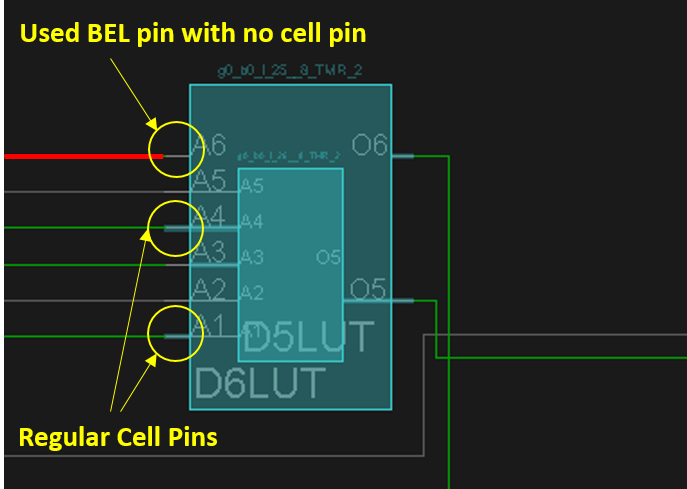
\includegraphics[width=.45\columnwidth]{pseudoCellPin.png}
  \caption{An example of VCC routing to an unused BEL pin (A6)}
  \label{fig:pseudoCellPin}
\end{figure}

To address this issue, RapidSmith2 allows users to create and attach
\texttt{PseudoCellPin}s to an existing cell. A \texttt{PseudoCellPin} is a
``fake'' cell pin that can be attached to a cell (after the cell has been
created), and then attached to a net to create a more complete view of the 
netlist. For example, a \texttt{PseudoCellPin} can be attached to the cell shown
in \autoref{fig:pseudoCellPin}, attached to the VCC net of the design, and then
mapped to the \texttt{A6} pin. Assuming the cell in the figure has the name of
``foo'', \autoref{lst:pseudoPin} demonstrates how to create and attach a new
\texttt{PseudoCellPin}.

\begin{lstlisting}[xleftmargin=1.5em, framexleftmargin=1.5em, caption=Required
function calls to attach a PseudoPin to a Cell, label=lst:pseudoPin] 
  // get a handle to a device and design
  CellDesign design = loadDesign();
  Device device = loadDevice();
  
  // get a handle to the appropriate cells, nets, and bel pins
  Cell cell = design.getCell("foo");
  CellNet vcc = design.getVccNet();
  BelPin bp = device.getSite("SLICE_X0Y179").getBel("D6LUT").getBelPin("A6");
  
  // create and attach the psuedo cell pin, and map it to the BelPin
  CellPin pseudo = cell.attachPseudoPin("VccTmpPin");
  vcc.connectToPin(pseudo);
  pseudo.mapToBelPin(bp);
\end{lstlisting}

\subsubsection {LUT Routethroughs} \label{sec:belRoutethroughs}
Besides their use in implementing logic equations, LUT BELs can also be
configured as PIPs in a fully-routed FPGA design (known as a routethrough). A
LUT is marked as a routethrough when its configuration equation,
\texttt{CONFIG.EQN}, maps the value of a single input pin directly to the
output pin. For timing, the A6 pin is the most preferable option for
a routethrough since it is the fastest, but pins A1-A5 can also be
used in cases of routing congestion. Routethrough LUTs are not explicitly
represented in a design netlist since there is no cell placed on the
corresponding BEL. Figure \ref{fig:routethroughs} shows two example routethrough
LUTs in Vivado. As described in Section~\ref{sec:routing}, routethroughs are
represented in RapidSmith2 with specific \texttt{Connection} objects, and can be
used when routing a net.

\begin{figure}[h]
  \centering
  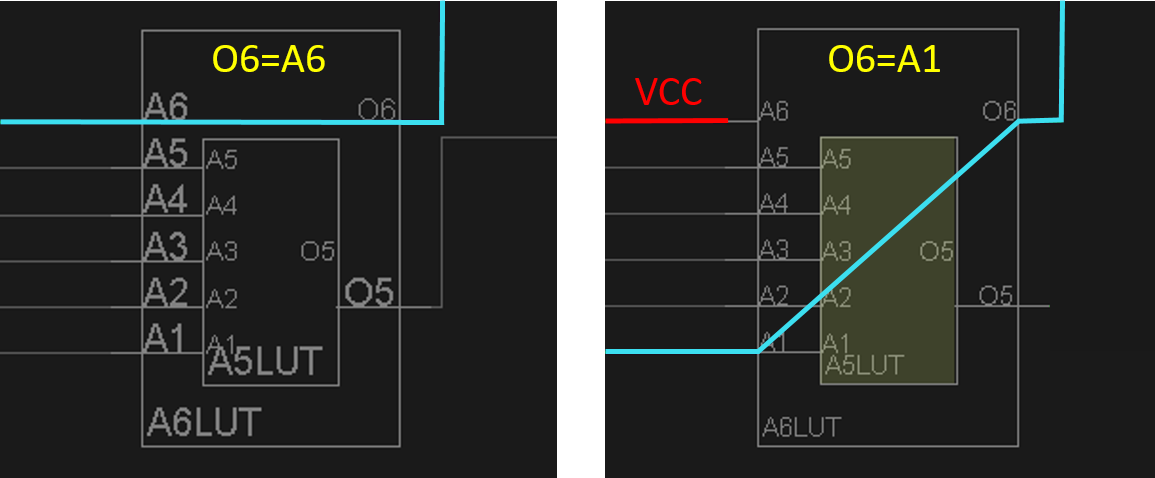
\includegraphics[width=5in]{routethroughs2.png}
  \caption{Two examples of LUTs configured as routethroughs in Vivado. The net
  highlighted in red represents VCC.}
  \label{fig:routethroughs}
\end{figure}

\subsubsection {Permanent Latches}

\begin{figure}[b!]
  \centering
  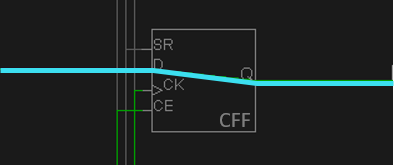
\includegraphics[width=.5\columnwidth]{ffRoutethrough.png}
  \caption{Flip-Flop BEL Configured as a Permanent Latch in Vivado}
  \label{fig:ffRoutethrough}
\end{figure}

A \textbf{permanent latch} in Vivado is a Flip Flop (FF) BEL which has been
configured as a latch with its ``set'' signal tied to VCC. This means that the
data pin of the latch always passes its value to the output pin of the latch,
and no state is retained. An example is shown in \autoref{fig:ffRoutethrough}.
As the figure shows, permanent latches look very similar to LUT routethroughs
described in the previous section. Because of this similarity, RapidSmith2
treates permanent latches the same as LUT routethroughs.

\subsubsection{Static Source LUTs}
Similar to their use as routethroughs, LUT BELs can also be configured as GND or
VCC signal sources. Examples of both are shown in
\autoref{fig:lutStaticSources}. The LUT on the left of the figure drives a VCC
signal and the LUT on the right drives GND. In both cases, the logical
netlist of a design does not represent the use of these LUTs in any way.
RapidSmith2 does explicitly represent static source LUTs. Like other VCC and GND
sources, they are implied based on where a VCC/GND route begins.

\begin{figure}[h]
  \centering
  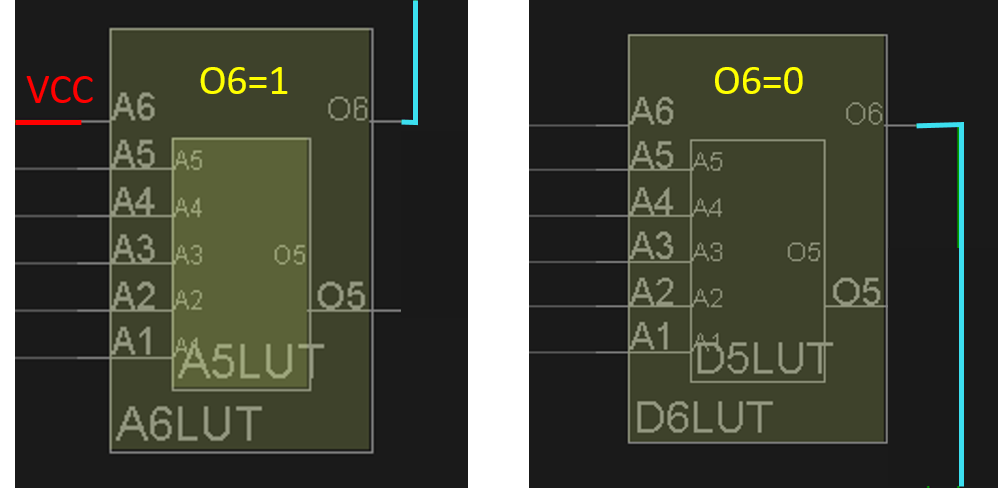
\includegraphics[width=.7\columnwidth]{lutStaticSources.png}
  \caption{Two LUTs Configured as Static Sources in Vivado}
  \label{fig:lutStaticSources}
\end{figure}

\vspace{-.2in}

\subsubsection{Site PIPs}
\begin{figure}[b!]
  \centering
  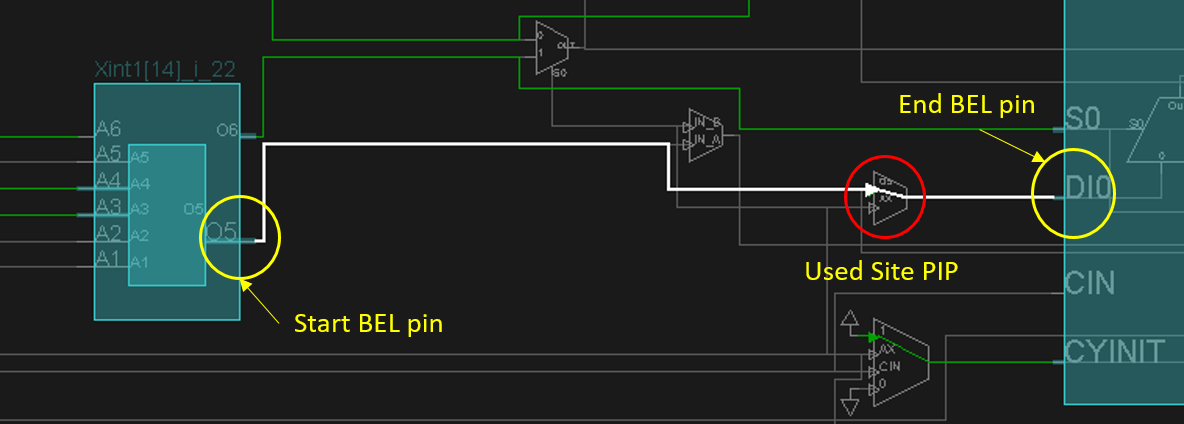
\includegraphics[width=\columnwidth]{sitePips.png}
  \caption{Site PIP Usage}
  \label{fig:sitePips}
\end{figure}

The internal routing structure of nets inside Vivado sites are represented by
a set of used site PIPs. A string of site PIPs enables a connection between site
components. An example is shown in \autoref{fig:sitePips} where the used site
PIPs are circled in red. As can be seen, the \texttt{ACY0:05} site PIP is
enabled and connects the \texttt{05} pin of the \texttt{A5LUT} BEL to the
\texttt{DI0} pin of the \texttt{CARRY4} BEL. Site PIPs can also be used to 
connect site pins to BEL pins. In RapidSmith2, a list of used site PIPs is
stored for each site on design import. The function call
\texttt{CellDesign::getUsedSitePipsAtSite(Site)} can be used to obtain the used
site PIPs at a given site location. Note that if your CAD program changes 
the cells placed in a site or the routing inside a site, it is your
responsibility to update this data structure accordingly.  For additional
details see the function \texttt{CellDesign::setUsedSitePipsAtSite(Site,
Set<Integer>)}.

\subsubsection{Site Properties}
Some properties not only affect how a Cell is configured, but they can also
affect how a Site is configured. For example, on SLICEL sites there exists a
clock routing mux that chooses between a regular clock signal and an inverted
signal (\autoref{fig:clkInv}). The output of this inverter is connected to all
flip flops of the SLICEL, and decides whether \textit{all} flip flops are
rising or falling-edge triggered. The clock that is selected is determined
by the property ``IS\_C\_INVERTED'' \textbf{of the flip flops cells that have
been placed onto the SLICEL}. The clock inverter is programmed automatically based on
the cell properties. There are other such properties, but they will not be listed
here. When creating designs in RapidSmith2, it is important to not place cells
together that may have conflicting properties. RapidSmith2 does not perform any
error checking, and so an error in Vivado will be thrown if you violate
property restrictions.

\begin{figure}[h!]
  \centering
  \includegraphics[width=.8\columnwidth]{clkInv.png}
  \caption{SLICEL clock inverter mux.}
  \label{fig:clkInv}
\end{figure}

%%%%%%%%%%%%%%%%%%%%%%%%%%%%%%%%%%%%%%%%%%%%%%%%%%%
% 	The Cell Library
%%%%%%%%%%%%%%%%%%%%%%%%%%%%%%%%%%%%%%%%%%%%%%%%%%%
\subsection{The Cell Library} \label{sec:cellLibraryinDesignSection}
As described in Section~\ref{sec:xilinxNetlist}, Xilinx netlists are composed of
cell objects which are instanced from backing library primitives. The most
common library primitives used in a Xilinx netlist include LUT (LUT1,
LUT2, etc) and Flip-Flop (FDRE, FDCE, etc.) cells. A detailed knowledge of the
available library cells for a device is required to perform any useful netlist
modification in external tools. To provide this information, \texttt{Tincr}
defines a \textbf{cell library XML}. A cell library contains the
following information for each library cell that can target a specific device:

\begin {itemize}
  \item Type
  \item Group (i.e. SLICE, DSP, IOB, BRAM, etc.) 
  \item Name, direction, and type for each library cell pin
  \item Valid placement locations for instances of the library cell
  \item Default logical-to-physical pin mappings for each cell pin
  \item Configurable properties with default values
  \item Macro templates 
\end{itemize}

RapidSmith2 parses the cell library XML file described above into a
\texttt{CellLibrary} data structure. This data structure is very useful when
performing any type of netlist manipulation or addition. Currently, each \texttt{CellLibrary}
corresponds to a specific Xilinx part. This means that for each device file in
RapidSmith2, a new \texttt{CellLibrary} needs to be generated \footnote{This may
change to be family-specific in the future.  We have observed that, usually,
parts in the same family can use the same \texttt{CellLibrary}.  But, for now
we recommend generating a new one for each device you use}.
\autoref{code:cellLibrary} shows two ways to load a \texttt{CellLibrary} in RapidSmith2. The following
subsections detail important aspects of a cell library.

\begin{lstlisting}[xleftmargin=1.5em, framexleftmargin=1.5em, caption=
Loading a CellLibrary in RapidSmith2, label=code:cellLibrary] 
// First way, load a Tincr Checkpoint
VivadoCheckpoint vcp = VivadoInterface.loadRSCP("checkpoint.rscp");
CellLibrary libCells1 = vcp.getLibCells();

// Second way, directly load the cell library from disk
CellLibrary libCells2 = new CellLibrary(RSEnvironment.defaultEnv()
                       .getPartFolderPath("xc7a100t-csg324-3")
                       .resolve("cellLibrary.xml");
\end{lstlisting} 

\subsubsection{Generating A New Cell Library} \label{sec:cellLibraryGeneration}
The \texttt{Tincr} command \texttt{[tincr::create\_xml\_cell\_library]} can be
used to generate a new cell library for a device. Specifically, follow the steps
listed below to create a new cell library (the items marked with
\textbf{SERIES7} only need to be done for series7 families).

\begin{enumerate}
  \item Open Vivado in Tcl mode, and run the command shown in the listing below.
  Replace ``xc7a100tcsg324-3'' with the part you want to generate and
  ``mycellLibrary.xml'' with the location where you want to store the generated
  cell library XML. This will generate most of what you need in the cell
  library XML automatically.
\end{enumerate}

  \begin{lstlisting} [numbers=none,keywordstyle=\ttfamily]
  Vivado% ::tincr::create_xml_cell_library xc7a100tcsg324-3 mycellLibrary.xml
  \end{lstlisting}

\begin{enumerate}
 \setcounter{enumi}{1} 
  \item \textbf{SERIES7}: Open the generated XML file in a text editor and
  search for the ``CARRY4'' cell. Scroll down to the ``bels'' XML element within
  the CARRY4 cell, and add the following lines to each pin that is named ``CI'':
  
  \begin{figure}[H]
   \centering
   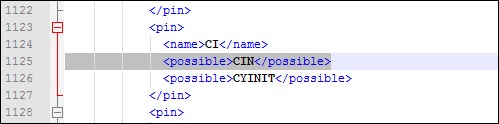
\includegraphics[width=.9\columnwidth]{cellLibHandEdit.png}
  \end{figure}
  
  You should have to insert this line in two places only.
  \item \textbf{SERIES7}: Save your changes and exit the text editor
  \item Copy the XML file to \textit{RapidSmithPath/device/family}
  directory where ``family'' is replaced by the family of your part (such as
  artix7), and ``RapidSmithPath'' is the location of your RapidSmith repository.
  Once this is complete the new \cls{CellLibrary} should be ready to use. 
\end{enumerate}

\subsubsection{Adding Custom Macros to a Cell Library} \label{sec:customMacros}
Customized, user-defined macros can be added to a RapidSmith2 \cls{CellLibrary}
if desired. This can be accomplished in two easy steps. 

\begin {enumerate}
  \item Create an XML specification
  of your macro that follows the format laid out in \autoref{lst:macroXml}.
\end {enumerate}

\begin{lstlisting}[language=XML, numbers=none, keywordstyle=, stringstyle=,
label=lst:macroXml, caption=Sample Macro XML for a CellLibrary] 
<?xml version="1.0" encoding="UTF-8"?> <root>	
  <macros>    
		<macro>
        <type>RAM128X1D</type>
        <!-- List of internal cells with name and leaf type of each -->
        <cells>
            <internal>
                <name>DP.HIGH</name>
                <type>RAMD64E</type>
            </internal>
            <internal>
                <name>DP.LOW</name>
                <type>RAMD64E</type>
            </internal>
            <internal>
                <name>F7.DP</name>
                <type>MUXF7</type>
            </internal>
			...
        </cells>
        <!-- List of macro pins with name, direction, pin type, and internal connections --> 
        <pins>
            <pin>
                <name>DPO</name>
                <direction>output</direction>
                <type>MACRO</type>
                <internalConnections>
                    <pinname>F7.DP/O</pinname>
                </internalConnections>
            </pin>
            <pin>
                <name>SPO</name>
                <direction>output</direction>
                <type>MACRO</type>
                <internalConnections>
                    <pinname>F7.SP/O</pinname>
                </internalConnections>
            </pin>
            <pin>
                <name>A[6]</name>
                <direction>input</direction>
                <type>MACRO</type>
                <internalConnections>
                    <pinname>F7.SP/S</pinname>
                    <pinname>DP.HIGH/WADR6</pinname>
                    <pinname>DP.LOW/WADR6</pinname>
                    <pinname>SP.HIGH/WADR6</pinname>
                    <pinname>SP.LOW/WADR6</pinname>
                </internalConnections>
            </pin>
            ...
        </pins>
        <!-- List of internal nets, and the internal cell pins they connect to --> 
        <internalNets>
            <internalNet>
                <name>DPO0</name>
                <pins>
                    <pinname>F7.DP/I0</pinname>
                    <pinname>DP.LOW/O</pinname>
                </pins>
            </internalNet>
            ...
        </internalNets>
    </macro>
	...
  </macros>
</root>
\end{lstlisting}

\begin{enumerate}
 \setcounter{enumi}{1} 
  \item Import the macro into the \cls{CellLibrary} using the API call shown in
  \autoref{code:macroImport}.

\end{enumerate}

\begin{lstlisting}[caption=Adding new macros to the Cell Library,
label=code:macroImport] 
// Get a handle to a CellLibrary
CellLibrary libCells = getCellLibrary();

// Add the macros in an XML file.
libCells.loadMacroXML(Paths.get("myMacro.xml"); 
\end{lstlisting}

\noindent
Once this is complete, you can use your custom macro in a \cls{CellDesign} like
a normal cell.

